\chapter{Related Work}

\section{Machine Learning}
There are many classes problems that machine learning can be used to solve, such
as the following~\cite{introtoml}:

\begin{itemize}
  \item \textbf{Supervised Learning}: Predict a real valued output (regression)
    or select one of $C$ predefined categorical outputs (classification)
    for a given input vector. This also includes problems like anomaly detection,
    ranking, and regression.
  \item \textbf{Unsupervised Learning}: Find structure or regularity in a given
    set of input vectors. This includes problems like density estimation and 
    clustering
  \item \textbf{Reinforcement Learning}: Develop a policy that allows an agent
    to observe the state of its environment and take the actions that will 
    achieve a large cumulative reward in the long run~\cite{introtorl}.
\end{itemize}

ModelDB S+C can store operations and models for supervised
and unsupervised learning problems. Reinforcement learning, however, is out
of scope for this thesis.

For a supervised learning problems, suppose there is a dataset $\mathcal{D}$ that
consists of $n$ pairs of $(\textbf{x}^{(i)}, y^{(i)})$. There is a
pair for each $i \in \{{1...n}\}$. The $\textbf{x}^{(i)}$ are $p$-dimensional feature
vectors that decribe the $i^{th}$ example. So, $\textbf{x}^{(i)} \in \mathbb{R}^{p}$. 
$y^{(i)}$ is either the class label associated with the $i^{th}$ example or
the regression target for that example. That is, $y^{(i)} \in \{1...C\}$ for classification
and $y^{(i)} \in \mathbb{R}$ for regression. The $\textbf{x}^{(i)}$ vectors
can also be expressed as a $n \times p$ matrix $\textbf{X}$.

A machine learning model is a function $f(\textbf{x}; \boldsymbol{\theta})$ where
$\boldsymbol{\theta}$ is a vector of model parameters (e.g. the weights of a linear regression
model or the encoded splits of a decision tree model). This function accepts an 
input vector $\textbf{x} \in \mathbb{R}^{p}$ and produces a real output (e.g. for regression)
or probability of being in a specific class (e.g. for classification).

When training a model, it is useful to split the dataset $\mathcal{D}$ into
a training set $\mathcal{D}_{train}$ and testing set $\mathcal{D}_{test}$. This ensures
that the model is evaluated on data it has not seen before. An objective function
$J(\boldsymbol{\theta}, \mathcal{D}_{train})$ is defined and $\boldsymbol{\theta}$ 
is chosen to maximize (or minimize, depending on the formulation) the objective function.

Machine learning also requires some hyperparameters (e.g. maximum depth of decision tree, regularization constant) 
to be set in order to guide the training of the model. One way to pick values for the hyperparameters
is to use a validation set. That is, the dataset $\mathcal{D}$ is broken into three pieces, 
$\mathcal{D}_{train}$, $\mathcal{D}_{validation}$, and $\mathcal{D}_{test}$. For each 
hyperparameter configuration, a model is trained on $\mathcal{D}_{train}$. Then, the model
is evaluated on $\mathcal{D}_{validation}$. Then, the chosen hyperparameter configuration
is the one that yielded the model that performed best on the validation set. 
Using a technique called cross validation can make better use of the data. In 
$k$-fold cross validation, $\mathcal{D}_{train}$ is broken into $k$ pieces (or folds) of roughly
equal size. Then, for a given hyperparameter configuration, a total of $k$ models are trained, each 
trained on all but one of the folds. Each model is evaluated on the fold that was left out,
and the resulting evaluation metrics are aggregated (e.g. averaged) to produce the evaluation
metric for the hyperparameter configuration. The hyperparameter configuration with the
largest evaluation metric is chosen as the best hyperparameter configuration. Then, a final
model is trained on the entire $\mathcal{D}_{train}$ and is then evaluated on $\mathcal{D}_{test}$ 
\cite{deeplearningbook}.

While the above concepts are not exhaustive, they provide an overview of machine learning that is sufficient to
understand the model building process and ModelDB S+C.

\section{Linear and Tree Models}
ModelDB S+C has special support for linear regression, logistic regression, 
decision tree, random forest, and gradient boosted tree models. Therefore, it is worth discussing
these models briefly.

A linear regression model is a function $f(\textbf{x}; \boldsymbol{\theta}) = \boldsymbol{\theta}^{T}\textbf{x}$,
where $\boldsymbol{\theta} \in \mathbb{R}^{p}$. Requiring that all feature vectors have an first entry of 
1 allows the model to incorporate an intercept term.

A logistic regression model is not actually used for regression, it is used for 
binary ($C=2$) classification. Under appropriate assumptions, the logistic 
regression model aims to predict the likelihood that a given input feature vector
belongs to class 1. Concretely, the logistic regression function is: 
$f(\textbf{x}; \boldsymbol{\theta}) = \frac{\exp{\boldsymbol{\theta}^{T}\textbf{x}}}{1 + \exp{\boldsymbol{\theta}^{T}\textbf{x}}}$.
Its output lies between 0 and 1.

A decision tree model partitions the input space into non-overlapping regions, where all
points in the same region are assigned the same value. This value could be a class label
in the case of classification or a real value in the case of regression. For a given input vector,
the decision tree considers a different feature at each internal node. The input vector is forwarded
to a child node based on the value of the feature. This child node, if it is an internal node, then considers another
feature and performs the same process. Eventually, the input vector arrives at a leaf node. Each leaf node corresponds to
a region of the input space, and thus has an associated value (e.g. class label or real number), which is taken
to be the prediction for the input vector. An illustration of this is shown in Figure \ref{fig:sample_decision_tree}.

\begin{figure}
  \centering
  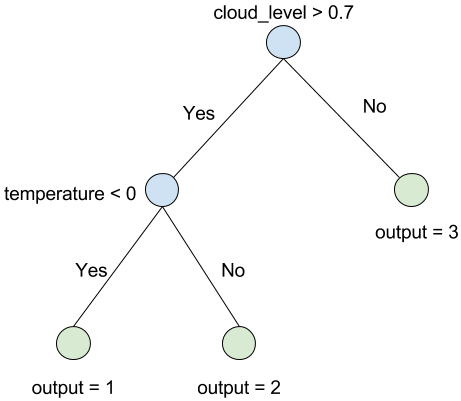
\includegraphics[height=3.0in]{sample_decision_tree}
  \caption{This is a decision tree model that could be used to predict whether the
  weather will be snowy (output 1), rainy (output 1), or neither (output 2) by
  looking at the cloud cover and temperature. The tree first checks if the cloud cover
  is high. If not, then it predicts there will be neither rain nor snow. Otherwise, the
  tree checks if the temperature is below 0. If so, then it predicts snow. Otherwise, it
  predicts rain.}
  \label{fig:sample_decision_tree}
\end{figure}

Random forest models and gradient boosted tree models are both ensembles of decision trees. They just differ in how they
are trained and applied. A random forest model trains many trees in parallel, where each tree is trained on a different bootstrapped
sample of the original dataset and where each split is only allowed to consider a subset of the features. A gradient boosted tree model
trains decision trees iteratively, where each successive decision tree learns to correct the mistakes of the previous trees. Like decision
trees, random forest and gradient boosted tree models can be used for both classification and regression. \cite{introtostatlearn}

These are not the only linear and tree models that are used in practice, but they are models that are supported in Spark.ML. 
Therefore, ModelDB S+C provides additional functionalty for the aforementioned models.

\section{Spark.ML}
Apache Spark \cite{spark} is a cluster computing engine that efficiently performs distributed computation
on data stored in-memory on many different machines. It is built around 
an abstraction called the Resilient Distributed Dataset (RDD). An RDD represents a dataset, its lineage,
and its partitioning. By tracking a dataset's lineage, an RDD allows the dataset to be recreated if it is
lost, thus providing fault tolerance. By tracking the partitioning and lazily performing operations, Spark
uses RDDs to schedule operations intelligently and pipeline them for efficiency.

Spark includes a number of libraries, two of which are relevant for this thesis. The first is Spark SQL,
which builds an abstraction called a DataFrame on top of the RDD abstraction. A DataFrame is simply a table
of data with named, typed columns. The second library
is Spark.ML, which lets users build machine learning models using Spark. Spark.ML lets the user create Transformers
that take an input DataFrame and produce an output DataFrame. It lets users use Estimators, which accept hyperparameters
and a DataFrame and produce a resulting model, which is simply a Transformer. Finally, Spark.ML provides a number
of other classes to support common model building tasks like cross validation and making preprocessing pipelines.

ModelDB S+C is built on three primitives: Transformer, DataFrame, and TransformerSpec, which are all inspired
by Spark SQL and Spark.ML. Transformer and DataFrame match their Spark counterparts, but unlike a Spark Estimator, a 
TransformerSpec simply describes how to create a model, rather than containing the logic for actually training the model.
ModelDB S+C does not train models, so there is no need for it to have model training logic.

The three primitives above, when coupled with ModelDB S+C's Syncable Event abstraction, can express a wide range
of model building operations.

The ModelDB Spark Client is a library designed for Spark.ML. It allows the user to use their existing
Spark.ML code, and with a few minor changes, store all their operations and models in ModelDB Server. 

\section{Machine Learning Libraries}
Since ModelDB Server aims to be library agnostic, it is worth looking at some other popular
machine learning libraries and understanding their abstractions for the model building process.

\subsection{MLI}
MLI \cite{mli} is an API for distributed machine learning. It includes an MLTable abstraction
that is very similar to the DataFrame abstraction in ModelDB S+C. MLI includes two other
tabular abstractions, the LocalMatrix and MLNumericTable, which are more restrictive forms of the
MLTable. MLNumericTable and LocalMatrix make computation easier, but they do not add anything to
the expressive power of MLI.

MLI's Optimizer and Algorithm abstractions help specify the logic for training a model. However,
as stated before, ModelDB S+C does not perform any training of models and thus these abstractions
are not important in the context of ModelDB S+C. That being said, the user can store information
about the algorithms and optimizer used to train a model in the hyperparameters of the model's associated
TransformerSpec.

MLI's Model abstraction maps to the Transformer abstraction in ModelDB S+C. There are two 
key differences between these abstractions. First, a Transformer is more general 
than a Model; it can represent data preprocessors as well as models. Second, a Model
stores the logic for making predictions while a Transformer does not. This is because
ModelDB S+C does not aim to make predictions, just to store and analyze the model building process. However,
the user is able to store serialized models in ModelDB S+C, which can later be deserialized and used to make
predictions.

\subsection{Scikit-learn}
Scikit-learn \cite{scikitlearn} is a machine learning library for Python. It expects data to
be given as matrices (two dimensional arrays in the numpy Python library) and DataFrames (from the Python
Pandas library). Both of these abstractions map nicely to ModelDB S+C's DataFrame.
A matrix can be thought of a DataFrame where all columns are numeric and where the column names are ignored.

Scikit-learn includes the concept of an Estimator, which contains logic for training a model and stores the hyperparameters.
This maps well to ModelDB S+C's TransformerSpec. The logic for training the model is not necessary for ModelDB S+C. Scikit-learn
also includes Transformer and Predictor concepts. The former is almost identical to ModelDB S+C's Transformer abstraction while the 
latter is simply a more restrictive kind of Transformer.

Finally, Scikit-learn includes abstractions for cross validation and pipelines, much like Spark.ML does. Both of these
model building tasks are represented in ModelDB S+C as Syncable Events.

\subsection{Weka}
Weka \cite{weka} is a machine learning toolkit that includes a user interface targeted for non-expert users.
It represents data as tables, which is very similar to ModelDB S+C's DataFrame.
However, Weka does not include separate abstractions for describing a model and describing the fitting of a model. Instead,
it combines them together in an abstraction called a Scheme. Thus, ModelDB S+C's TransformerSpec and Transformer abstraction
together reflect the same information as a Weka Scheme. Finally, Weka includes pre-processing and post-processing utilities which
map well to ModelDB S+C's Transformer abstraction.

\subsection{Pylearn 2}
Pylearn 2 \cite{pylearn2} is a machine learning library geared towards researchers. It includes the concept of a Dataset, Model,
and TrainingAlgorithm, which are analogous to ModelDB S+C's concepts of a DataFrame, Transformer, and TransformerSpec.
ModelDB S+C's Transformer abstraction is more general than a Model because it can capture both models as well as data preprocessors.
Pylearn 2 also includes abstractions such as Cost and TerminationCriterion. Since ModelDB S+C does not concern itself with the
details of training models, it has no corresponding abstractions and instead allows the data scientist to specify cost and termination criterion
as hyperparameters in a TransformerSpec.

\subsection{Tensorflow}
Tensorflow \cite{tensorflow} is machine learning library that allows users to specify computation graphs, which is
especially useful for training neural network models. It represents data in the form of a Tensor. 
This is actually more general than the DataFrame concept in ModelDB S+C. However, using a tensor abstraction in ModelDB S+C may
add a good deal of complexity to the other abstractions without enabling a great deal of new functionality. 

Tensorflow represents data in the form of a computation graph, where nodes 
called variables use operations along edges to send tensors through the graph.
ModelDB S+C stores a graph, specified by the TransformEvents, where the 
nodes are DataFrames and the edges are Transformers. Tensorflow's computation 
graph is useful for performing efficient training of models. However, since 
ModelDB S+C does not actually do any training of models and instead just 
captures operations like transformations and model-fitting, its graph is 
different than TensorFlows. Additionally, Tensorflow requires the user to 
specifiy their computation graph up-front in order for
the library to determine how to train the model. ModelDB S+C, on 
the other hand, builds up its graph over time as the user performs operations.

\subsection{Summary}
Thus, ModelDB S+C's abstractions seem to be general enough that there are analogs
in a number of other machine learning libraries. Of the examples above, Tensorflow
is the only one with a significantly different set of abstractions than ModelDB S+C.

\section{Model Building Support Systems}
ModelDB S+C does not actually train any machine learning models and it does not 
make any predictions. Rather, it collects, stores, and analyzes data about 
the model building process. In this way, ModelDB S+C supports the process of
model building rather performing the process itself. This section describes
other systems which support the model building process.

\subsection{ModelHub}
ModelHub \cite{modelhub} is similar to the overall ModelDB system in that it also
aims to to provide a suite of systems like model version control, a command line
toolkit, and a model exploration API, to support the model building process. ModelHub
focuses on deep learning and provides specialized tools for that domain, however, 
while ModelDB is aimed at machine learning models in general. Additionally, while
ModelHub tracks changes made to models, it does not track transformations 
made to datasets like ModelDB S+C does. Finally, ModelHub does not describe
any client libraries or abstractions that allow collecting data about the data
scientist's operations as they are performed. ModelDB Spark Client, on the other hand,
records a wide range of machine learning operations, like random splitting of datasets,
annotating datasets, and creating preprocessing pipelines, as the user does them and
stores them in ModelDB Server.

\subsection{MLDB}
MLDB \cite{mldb} is a system that allows users to create and store machine learning
models as well as datasets in a central database and access them through a REST API. 
While it supports the storage of models, it does not store operations (e.g. random splitting,
pipeline creation) that the user performs. Additionally, there are no client libraries
that can record these operations behind the scenes and send them to the server with
minimal user involvement. Finally, MLDB does not offer an API for querying operations
and gleaning information from them.

\subsection{Azure ML}
Microsoft's Azure Machine Learning \cite{azureml} is a cloud service that allows users
to create machine learning models with a web interface, store them in the cloud, and
access them via web service. Azure Machine Learning requires users to construct a dataflow 
graph indicating their full pre-processing and model training operations before model building
happens. ModelDB S+C, on the other hand, does not ask the user to indicate their full model building
workflow beforehand, and will instead record the operations and models as they appear. ModelDB Server
focuses on storing and analyzing the model building process and allows the user to use another library
(Spark.ML in this thesis) for training models. Azure Machine Learning, on the other hand, requires
that the user use its model training system. Finally ModelDB Spark Client works with a user's existing
Spark.ML code, allowing them to log their operations and models with few code changes. Azure Machine
Learning, on the other hand, requires users to convert significant parts of their code into
dataflow graphs using its proprietary user interface.

\subsection{Velox}
Velox \cite{velox} is a system for low latency serving and management of machine learning models.
While it does support storage of models, it does not store operations performed in model building and it
does not expose APIs for analyzing the model building process.

\subsection{MLBase}
MLBase \cite{mlbase} is a database system with the ability to store and serve machine learning
models. It includes an optimizer that figures out a plan for training a model. Unlike ModelDB S+C,
it does not track and store the operations in the model building process. It also requires users to
specify their model building process using a declarative language with hints for the optimizer. While this
can be useful for non-experts, it reduces the control that a user has over their model building process.
ModelDB S+C on the other hand, only requires a few minor changes to the user's Spark.ML code in order to
store the data associated with the model building process.

\subsection{PMML}
PMML \cite{pmml} is an XML-like markup language for representing machine learning models. While it
can describe a wide range of machine learning models, it cannot represent general model building operations
like ModelDB Server's database does. It is not possible to run queries on PMML either, but ModelDB Server
exposes an API for querying model building operations and stores operation data in a SQL database. PMML can,
however, complement ModelDB Server because a user can choose to store their serialized models in PMML form.

\subsection{Longview}
Longview is a predictive DBMS. It allows users to store machine learning models in a relational database
and access them via a user defined function in their queries. Unlike ModelDB Server and Spark Client, it
cannot work with a user's existing code, and instead requires them to use Longview for all their
model training. Finally, Longview does not store machine learning operations like ModelDB Server does.
